\chapter[Revisão Bibliográfica]{Revisão Bibliográfica}
\label{chap:revisao}
\thispagestyle{empty}

Este capítulo é divido em duas seções que visam apresentar os conceitos necessários para a compreensão deste PFC.
Na primeira seção são apresentados conceitos para uma modelagem matemática da dinâmica de um veículo em baixas velocidades.
São apresentado na segunda seção uma introdução à teoria de controle ótimo e a utilização de \textit{software} na solução
de problemas de controle ótimo.

\section{Modelo do veículo}
\label{sec:modelo}

Um modelo matemático, ou apenas modelo, é um conjunto de equações que descreve de forma adequada o comportamento de um sistema que deseja-se estudar.
Uma forma usual de classificação dos métodos de modelagem é separá-los nas categorias: modelagem caixa branca, modelagem caixa preta e modelagem
caixa cinza.
A modelagem caixa branca, também conhecida como modelagem conceitual, consiste na aplicação princípios fundamentais e por isso exige um conhecimento
da natureza do sistema.
A modelagem caixa preta, ou modelagem empírica, é baseada na aplicação de técnicas de identificação de sistemas que exigem pouco ou
nenhum conhecimento do sistema.
Já na modelagem caixa cinza são utilizadas técnicas que estão entre a modelagem caixa branca e a modelagem caixa preta. \cite[Seç.~1.1]{book:Aguirre}

Nessa seção o método de modelagem aplicado é de modelagem caixa branca. A partir da aplicação da segunda lei de Newton no
veículo representado no diagrama da Figura \ref{fig:diag_forcas_veiculo}, obtém-se a equação que descreve a dinâmica longitudinal do mesmo

\begin{equation}
	\label{eq:SomaForcas}
	(m_v + m_p + m_r) \dot v = F_t - (F_a + F_g + F_r)
	\enspace,
\end{equation}

em que $m_v$ é a massa do veículo, $m_v$ é a massa do piloto,  $m_r$ é massa equivalente ao momento de inercia das partes rotativas (rodas e eixo do motor),  $v$ é a velocidade, $F_{t}$ é a propulsão feita pelo motor, $F_{a}$ é o
arrasto aerodinâmico, $F_g$ é a componente do peso que está direção da velocidade e $F_{r}$ é a resistência ao rolamento dos pneus na pista.
Os modelos que descrevem a massa equivalente $m_r$ e forças $F_{a}$, $F_g$, $F_{r}$ e $F_{t}$ estão apresentados nas subseções a seguir.

\begin{figure}[h]
	\centering
	\caption{Diagrama de forças de um veículo em movimento}
	\label{fig:diag_forcas_veiculo}
	\begin{normalsize}
		\import{DescricaoProcesso/Figuras/}{diagrama_forcas_veiculo.pdf_tex}
	\end{normalsize}
	\caption*{\footnotesize Fonte: Elaborado pelo autor.}
\end{figure}

\subsection{Inércia rotacional}

A inércia de todas as peças giratórias dentro do veículo causa forças fictícias. 
Está inércia pode ser representada nos modelos dinâmicos do motor e da transmissão, ou ser representada com uma massa equivalente $m_r$.
Para essa representação é considerado que não há deslizamento do pneu no asfalto e não há escorregamento na transmissão. O cálculo de $m_r$ é 

\begin{subequations}
	\label{eq:mr}
	\begin{align}
		m_r = m_{r,r} + m_{r,m} \enspace, \label{eq:mr1} \\
		m_{r,r} = \sum_{n=1}^{Nr} J_r \cdot \frac{1}{r_r^2} \enspace, \label{eq:mr2} \\
		m_{r,m} = J_m \cdot \frac{\varphi^2}{r_r^2} \enspace, \label{eq:mr3}
	\end{align}
\end{subequations}

em que $m_{r,r}$ é a massa equivalente a inércia das rodas e $m_{r,m}$ é a massa equivalente a inércia do motor, $Nr$ é a quantidade de rodas, 
$J_r$ e $r_r$ são o momento de inércia e o raio da roda, $J_m$ é o momento de inércia do motor e 
$\varphi$ é a relação de transmissão. \hbox{\cite[Seç.~2.1.1]{book:guzzella2012vehicle}}

\subsection{Arrasto aerodinâmico}
\label{subsec:arrasto_aerodinamico}

O movimento de um objeto imerso em um fluido sofre uma resistência causada por esse fluido. No
caso de veículos que se deslocam no ar, essa
resistência é chamada de arrasto aerodinâmico.
Pode-se aproximar o cálculo dessa força $F_{a}$ com a equação

\begin{equation}
	\label{eq:Fa}
	F_a(v) = \frac{\rho \cdot a_f \cdot c_d \cdot v^2}{2}
	\enspace,
\end{equation}

em que $v$ é a velocidade do veículo em relação à atmosfera, $\rho$ a densidade do ar, $a_{f}$ a área frontal do
veículo e $c_{d}$ o coeficiente de arrasto aerodinâmico.
O coeficiente $c_{d}$ é um numero adimensional e depende da geometria veículo, é determinado por meio de simulações em \textit{software} de fluido
dinâmica
computacional (CFD, do inglês \textit{computational fluid dynamics}) e/ou experimentos em túnel de vento. \cite[Seç.~2.1.1]{book:guzzella2012vehicle} Alguns
valores típicos de $c_{d}$ para diferentes tipos de
veículos são apresentados na Tabela \ref{tab:ComparacaoCD}.

\begin{table}[h]
	\centering
	\caption{Comparação do $c_{d}$ para diferentes tipos de veículos}
	\rowcolors{1}{}{lightgray}
	\begin{tabular}{ll}
		\toprule
		\textbf{veículo} & \boldsymbol{$c_{d}$} \\
		\hline
		Carro            & 0,3 - 0,4            \\
		Ônibus           & 0,6 - 0,7            \\
		Caminhão         & 0,6 - 1,0            \\
		Moto             & 0,5 - 1,0            \\
		\bottomrule
	\end{tabular}
	\caption*{\footnotesize Fonte: Adaptado de \citeauthoronline{book:GroundVehicleDynamics}. \cite[Seç.~8.3]{book:GroundVehicleDynamics}}
	\label{tab:ComparacaoCD}
\end{table}

\subsection{Relevo da pista}

A componente do peso, $F_{g}$, afeta consideravelmente a dinâmica do veículo e atua sempre que a pista não é plana. Seu modelo é a equação

\begin{equation}
	\label{eq:Fg}
	F_{g}(\theta) = (m_v + m_p) \cdot g \cdot \sin(\theta)
	\enspace,
\end{equation}

que, pra pequenas inclinações, pode ser aproximado pela equação

\[
	F_{g}(\theta) \approx  (m_v + m_p) \cdot g \cdot \theta
	\enspace,
\]


em que $m$ é a massa total do veículo, $g$ é a aceleração da gravidade e $\theta$ é a inclinação da pista expressa em
radianos. \cite[Seç.~2.1.1]{book:guzzella2012vehicle}

\subsection{Resistência ao rolamento}
\label{subsec:resistencia_rolamento}

A norma ISO 4223-1:2017 define a resistência ao rolamento de um pneu, como a energia consumida pelo pneu por unidade de distância 
percorrida. Esse consumo de energia se deve principalmente as propriedades viscoelásticas dos compostos de borracha presente no pneu.
Durante a rolagem o pneu é deformado na zona de contato entre o pneu e o pavimento, nessa zona de contato a resultante da força de reação à força
normal não
está no mesmo eixo que a força normal, Figura \ref{fig:diagramaPeneu}, de forma a gerar uma força, $F_{r}$, contraria a movimentação do pneu.

\tikzset{every picture/.style={line width=0.75pt}} %set default line width to 0.75pt        
\begin{figure}[H]
    \begin{center}
        \caption{Legenda diagrama pneu}
        \label{fig:diagramaPeneu}
        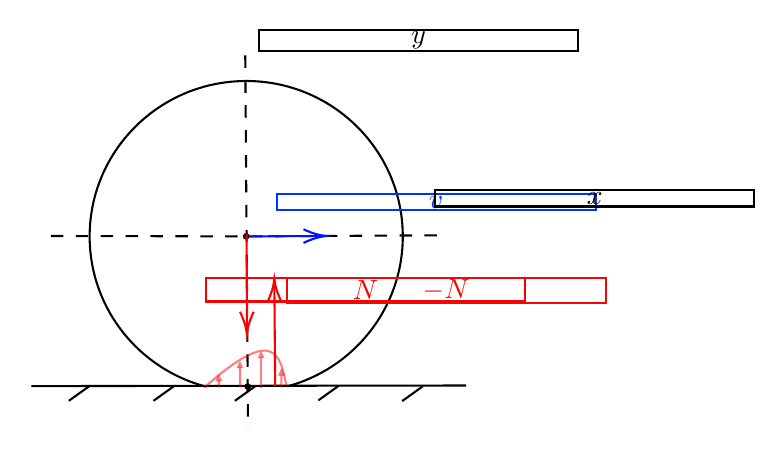
\begin{tikzpicture}[x=0.75pt,y=0.75pt,yscale=-1,xscale=1]
            %uncomment if require: \path (0,189); %set diagram left start at 0, and has height of 189

            %Straight Lines [id:da7518330174479086] 
            \draw  [dash pattern={on 4.5pt off 4.5pt}]  (6.67,90) -- (100.79,90.19) -- (193.33,89.67) ;
            %Straight Lines [id:da5592434503400421] 
            \draw	 (-2.68,162.32) -- (206.73,162.03) ;
            %Shape: Arc [id:dp1726281412706019] 
            \draw  [draw opacity=0][fill={rgb, 255:red, 8; green, 7; blue, 7 }  ,fill opacity=0 ] (81.65,162.63) .. controls (49.67,154.34) and
            (25.87,125.7) .. (25.36,91.3) .. controls (24.76,49.95) and (58.03,15.94) .. (99.69,15.33) .. controls (141.35,14.72) and (175.61,47.74) ..
            (176.22,89.08) .. controls (176.73,124) and (153.08,153.68) .. (120.62,162.44) -- (100.79,90.19) -- cycle ; \draw   (81.65,162.63) .. controls
            (49.67,154.34) and (25.87,125.7) .. (25.36,91.3) .. controls (24.76,49.95) and (58.03,15.94) .. (99.69,15.33) .. controls (141.35,14.72) and
            (175.61,47.74) .. (176.22,89.08) .. controls (176.73,124) and (153.08,153.68) .. (120.62,162.44) ;
            %Straight Lines [id:da003920177628984778] 
            \draw [color={rgb, 255:red, 4; green, 18; blue, 249 }  ,draw opacity=1 ]   (100.79,90.19) -- (137.33,90.01) ;
            \draw [shift={(139.33,90)}, rotate = 539.72] [color={rgb, 255:red, 4; green, 18; blue, 249 }  ,draw opacity=1 ][line width=0.75]
            (10.93,-3.29) .. controls (6.95,-1.4) and (3.31,-0.3) .. (0,0) .. controls (3.31,0.3) and (6.95,1.4) .. (10.93,3.29)   ;
            %Straight Lines [id:da6241641943206588] 
            \draw [color={rgb, 255:red, 0; green, 0; blue, 0 }  ,draw opacity=1 ]	(25.2,162.33) -- (15.33,169.4) ;
            %Straight Lines [id:da6421337551968986] 
            \draw [color={rgb, 255:red, 0; green, 0; blue, 0 }  ,draw opacity=1 ]	(66,162.33) -- (56.13,169.4) ;
            %Straight Lines [id:da25242184369144227] 
            \draw [color={rgb, 255:red, 0; green, 0; blue, 0 }  ,draw opacity=1 ]	(105.2,162.33) -- (95.33,169.4) ;
            %Straight Lines [id:da7965874493492349] 
            \draw [color={rgb, 255:red, 0; green, 0; blue, 0 }  ,draw opacity=1 ]	(145.4,162.13) -- (135.53,169.2) ;
            %Straight Lines [id:da2366122350933053] 
            \draw [color={rgb, 255:red, 0; green, 0; blue, 0 }  ,draw opacity=1 ]	(185.8,162.47) -- (175.93,169.53) ;
            %Straight Lines [id:da201352955590123] 
            \draw  [dash pattern={on 4.5pt off 4.5pt}]  (100.33,3) -- (101.67,183) ;
            %Straight Lines [id:da12037912623915337] 
            \draw	 (-4,15.67) ;
            %Shape: Circle [id:dp21540655765824446] 
            \draw  [color={rgb, 255:red, 0; green, 0; blue, 0 }  ,draw opacity=1 ][fill={rgb, 255:red, 0; green, 0; blue, 0 }  ,fill opacity=1 ]
            (100.45,162.53) .. controls (100.45,161.94) and (100.94,161.45) .. (101.53,161.45) .. controls (102.13,161.45) and (102.62,161.94) .. (102.62,162.53)
            .. controls (102.62,163.13) and (102.13,163.62) .. (101.53,163.62) .. controls (100.94,163.62) and (100.45,163.13) .. (100.45,162.53) -- cycle ;
            %Shape: Circle [id:dp5323977356859111] 
            \draw  [color={rgb, 255:red, 0; green, 0; blue, 0 }  ,draw opacity=1 ][fill={rgb, 255:red, 0; green, 0; blue, 0 }  ,fill opacity=1 ]
            (99.73,89.99) .. controls (99.84,89.4) and (100.4,89.01) .. (100.99,89.13) .. controls (101.58,89.24) and (101.97,89.8) .. (101.85,90.39) .. controls
            (101.74,90.98) and (101.17,91.37) .. (100.59,91.25) .. controls (100,91.14) and (99.61,90.58) .. (99.73,89.99) -- cycle ;
            %Straight Lines [id:da8962219135738276] 
            \draw [color={rgb, 255:red, 255; green, 0; blue, 0 }  ,draw opacity=1 ]   (100.99,89.13) -- (101.13,135.43) ;
            \draw [shift={(101.13,137.43)}, rotate = 269.83] [color={rgb, 255:red, 255; green, 0; blue, 0 }  ,draw opacity=1 ][line width=0.75]
            (10.93,-3.29) .. controls (6.95,-1.4) and (3.31,-0.3) .. (0,0) .. controls (3.31,0.3) and (6.95,1.4) .. (10.93,3.29)	;
            %Straight Lines [id:da7902625791767064] 
            \draw [color={rgb, 255:red, 246; green, 0; blue, 0 }  ,draw opacity=1 ][fill={rgb, 255:red, 254; green, 0; blue, 0 }  ,fill opacity=1
            ]   (114.73,162.23) -- (114.35,112.63) ;
            \draw [shift={(114.33,110.63)}, rotate = 449.56] [color={rgb, 255:red, 246; green, 0; blue, 0 }  ,draw opacity=1 ][line width=0.75]
            (10.93,-3.29) .. controls (6.95,-1.4) and (3.31,-0.3) .. (0,0) .. controls (3.31,0.3) and (6.95,1.4) .. (10.93,3.29)	;
            %Curve Lines [id:da9381909177646195] 
            \draw [color={rgb, 255:red, 255; green, 0; blue, 0 }  ,draw opacity=0.51 ]   (81.25,162.43) .. controls (115.59,132.01) and
            (117.14,148.45) .. (120.22,162.24) ;
            %Straight Lines [id:da46399317653073635] 
            \draw [color={rgb, 255:red, 255; green, 0; blue, 0 }  ,draw opacity=0.51 ]   (87.58,162.88) -- (87.55,159.32) ;
            \draw [shift={(87.53,156.32)}, rotate = 449.5] [fill={rgb, 255:red, 255; green, 0; blue, 0 }  ,fill opacity=0.51 ][line width=0.08]
            [draw opacity=0] (3.57,-1.72) -- (0,0) -- (3.57,1.72) -- cycle	  ;
            %Straight Lines [id:da977275191245905] 
            \draw [color={rgb, 255:red, 255; green, 0; blue, 0 }  ,draw opacity=0.51 ]   (97.93,162.92) -- (97.77,153.12) ;
            \draw [shift={(97.73,150.12)}, rotate = 449.1] [fill={rgb, 255:red, 255; green, 0; blue, 0 }  ,fill opacity=0.51 ][line width=0.08]
            [draw opacity=0] (3.57,-1.72) -- (0,0) -- (3.57,1.72) -- cycle	  ;
            %Straight Lines [id:da7569878460768078] 
            \draw [color={rgb, 255:red, 255; green, 0; blue, 0 }  ,draw opacity=0.51 ]   (107.93,163.12) -- (107.93,148.32) ;
            \draw [shift={(107.93,145.32)}, rotate = 450] [fill={rgb, 255:red, 255; green, 0; blue, 0 }  ,fill opacity=0.51 ][line width=0.08]
            [draw opacity=0] (3.57,-1.72) -- (0,0) -- (3.57,1.72) -- cycle	  ;
            %Straight Lines [id:da6646192752580227] 
            \draw [color={rgb, 255:red, 255; green, 0; blue, 0 }  ,draw opacity=0.51 ]   (117.78,162.93) -- (117.74,156.72) ;
            \draw [shift={(117.73,153.72)}, rotate = 449.64] [fill={rgb, 255:red, 255; green, 0; blue, 0 }	,fill opacity=0.51 ][line width=0.08]
            [draw opacity=0] (3.57,-1.72) -- (0,0) -- (3.57,1.72) -- cycle    ;

            % Text Node
            \draw (114.93,69.33) node [anchor=north west][inner sep=0.75pt]  [color={rgb, 255:red, 3; green, 49; blue, 254 }  ,opacity=1 ]
            {$v$};
            % Text Node
            \draw (80.93,109.93) node [anchor=north west][inner sep=0.75pt]  [color={rgb, 255:red, 249; green, 0; blue, 0 }  ,opacity=1 ]  {$N$};
            % Text Node
            \draw (119.73,109.53) node [anchor=north west][inner sep=0.75pt]  [color={rgb, 255:red, 247; green, 4; blue, 4 }  ,opacity=1 ]
            {$-N$};
            % Text Node
            \draw (191.33,67.53) node [anchor=north west][inner sep=0.75pt]    {$x$};
            % Text Node
            \draw (106.53,-9.87) node [anchor=north west][inner sep=0.75pt]    {$y$};

        \end{tikzpicture}
    \end{center}
    \caption*{\footnotesize Fonte: Elaborado pelo autor.}
\end{figure}


A força de resistência ao rolamento, $F_{r}$, depende da construção do pneu e do tipo de pavimento. Essa força também depende da velocidade do
veículo e da pressão do ar no pneu,
embora nesse trabalho não considera-se essa dependência. Para calculá-la usa-se a relação:

\begin{equation}
	\label{eq:Fr}
	F_{r}  = c_{r} \cdot N
	\enspace,
\end{equation}

em que $c_{r}$ é o coeficiente de resistência ao rolamento, $N$ é a força normal sobre o pneu e $F_{r}$ é a força
gerada pela resistência ao rolamento.
Estão apesentados na Tabela \ref{tab:ComparacaoCr}
o valor do coeficiente $c_{r}$ para pneus de uso típico em carros de passeio, bicicletas e de dois pneus específicos para a competição SEM,
Michelin
45-406 \textit{Prototype} e Michelin  Radial 45-75 R16.

% Escrever que nao vou conciderar pq nao da pra medir a variacao no cenario atual.
% Colocar como perpestivas de trabalho futuro.

\begin{table}[H]
	\centering
	\caption{Comparação do coeficiente $c_{r}$ de diferentes pneus}
	\rowcolors{1}{}{lightgray}
	\begin{tabular}{ll}
		\toprule
		\textbf{Pneu}                                                       &
		\boldsymbol{$c_{r}$}                                                          \\
		\hline
		Usado em carro                                                      & 0,013
		\\
		Usado em bicicleta                                                  & 0,006
		\\
		Michelin  45-406 \textit{Prototype} & 0,0024  \\
		Michelin  Radial 45-75 R16          & 0,00081 \\
		\bottomrule
	\end{tabular}
	\caption*{\footnotesize Fonte: Adaptado de  \citeauthoronline{book:PacCarII} \cite[Seç.~2.2.1]{book:PacCarII}.}
	\label{tab:ComparacaoCr}
\end{table}

% \begin{figure}[h]
% 	\centering
% 	\caption{Pneu Michelin  44-406 \textit{Prototype}}
% 	\label{fig:pneu}
% 	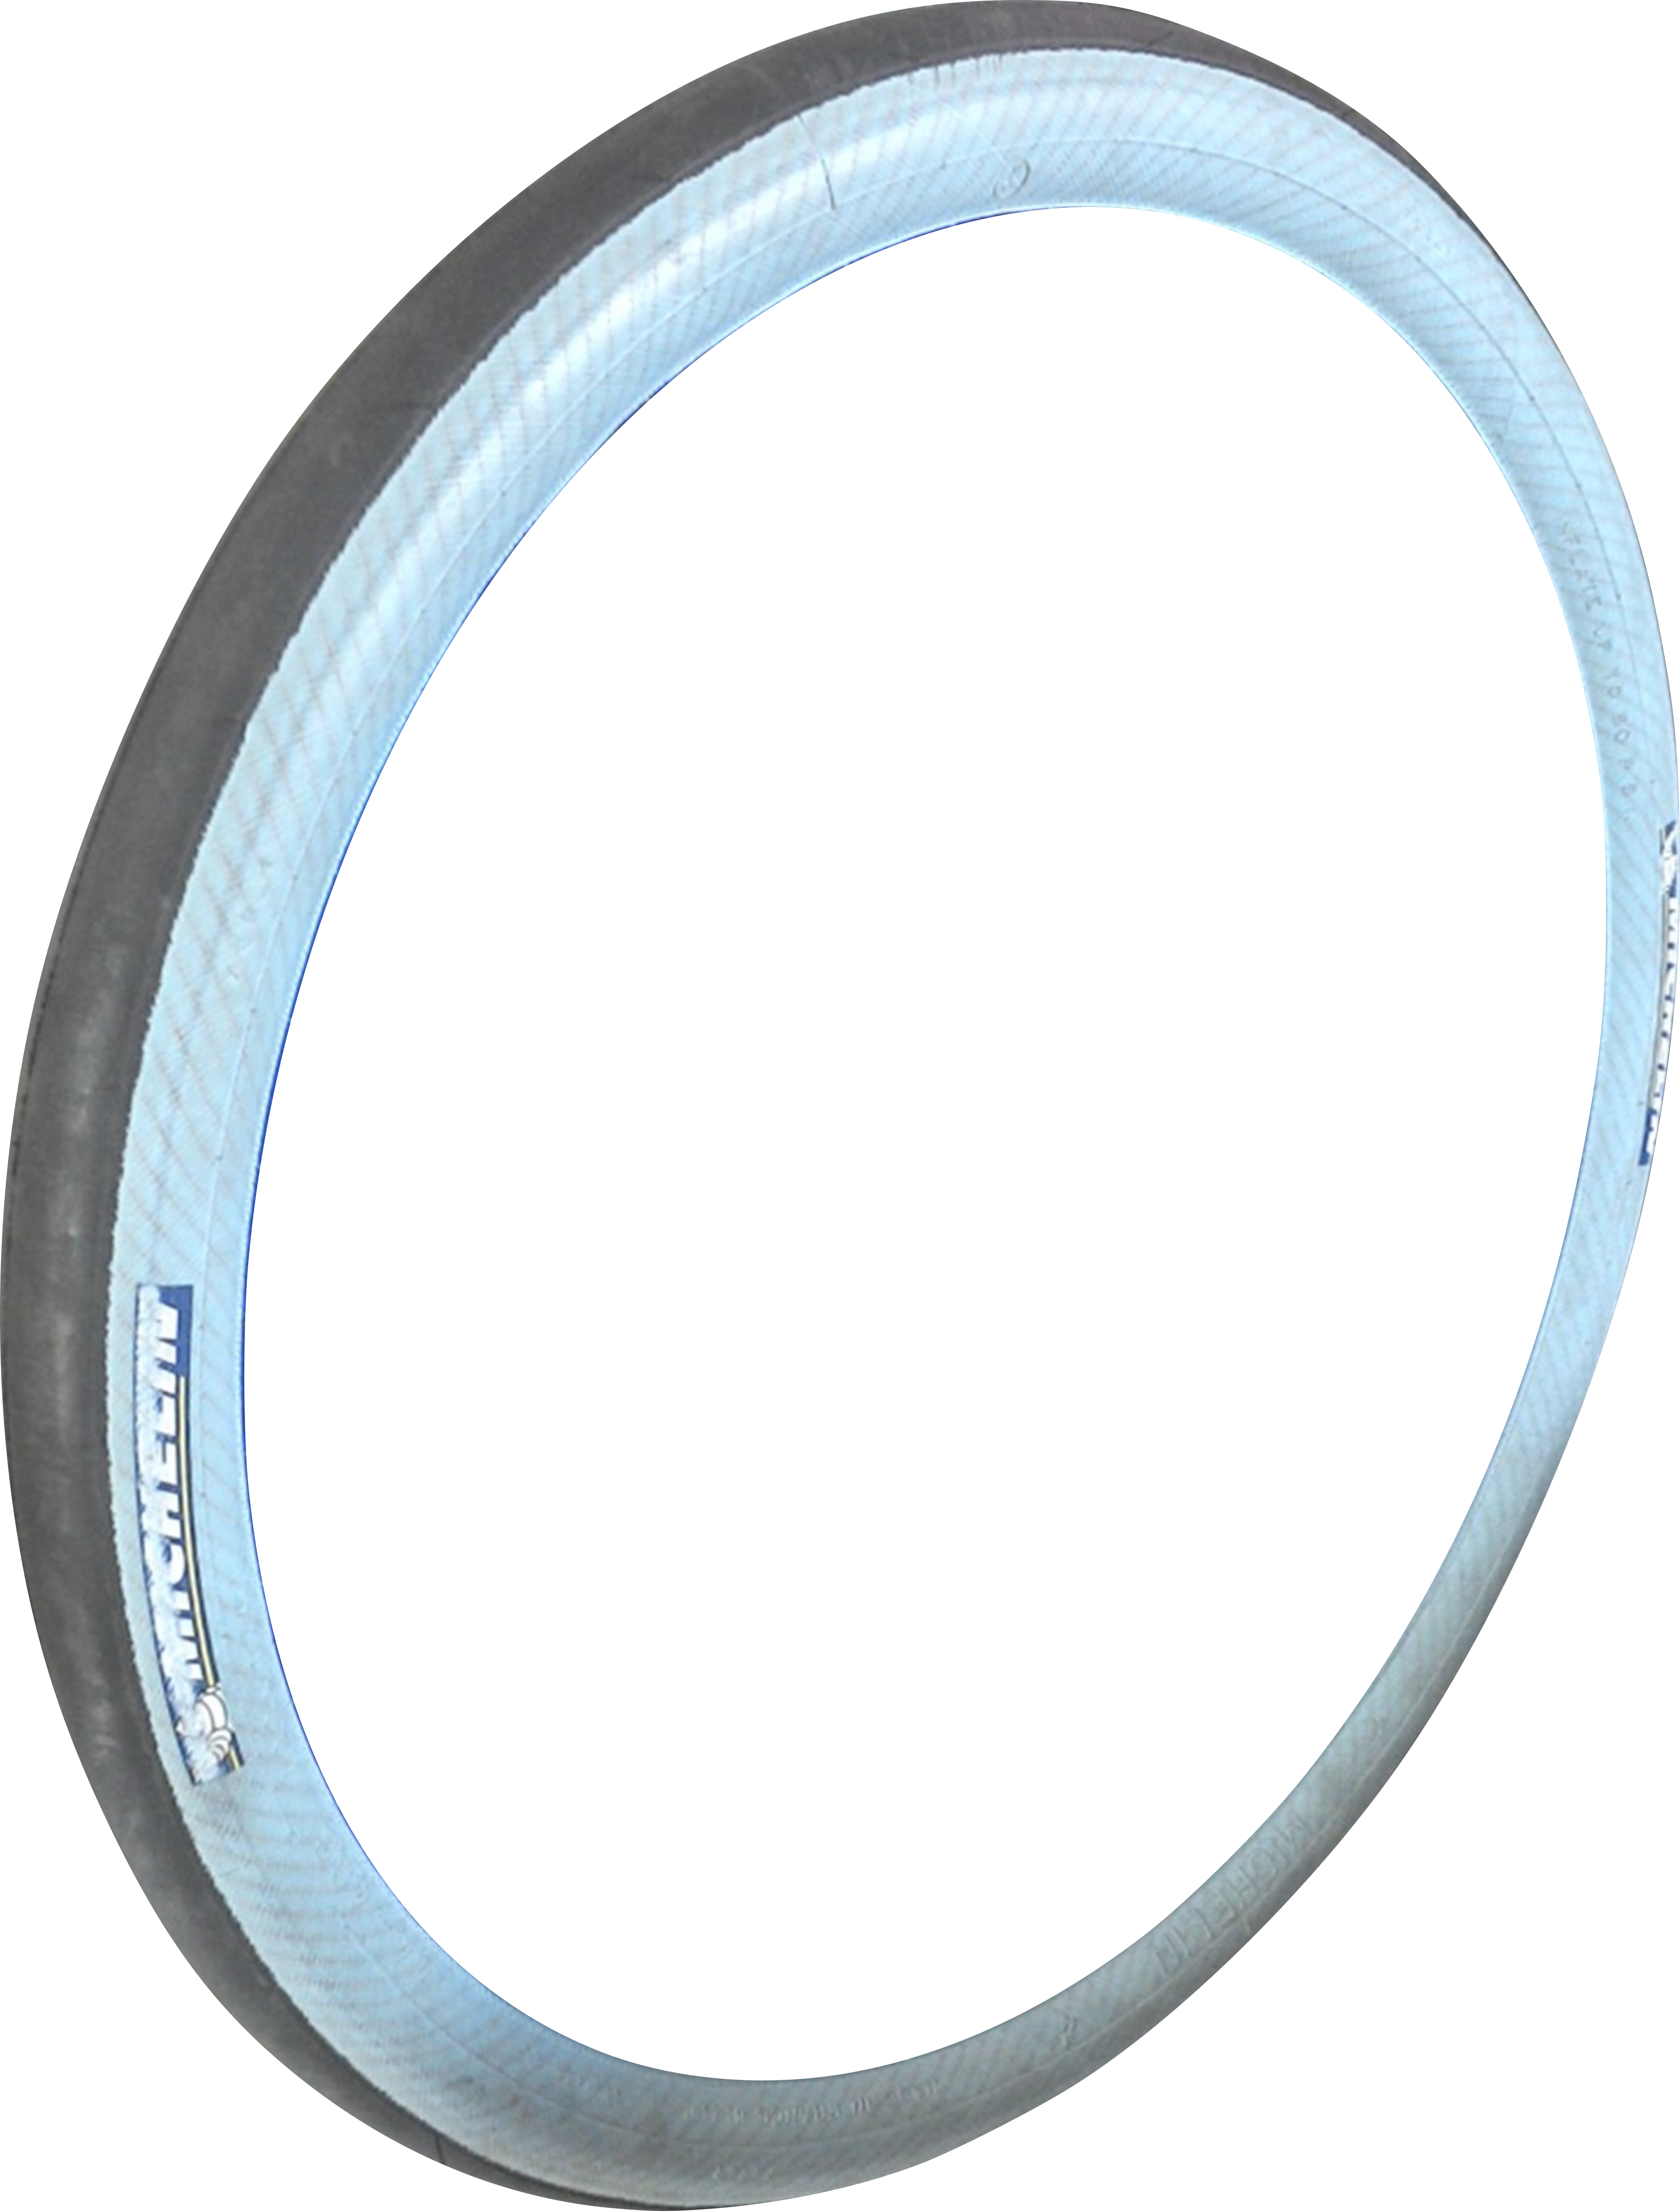
\includegraphics[scale=0.20]{DescricaoProcesso/Figuras/pneu_Michelin.png}
% 	\caption*{\footnotesize Fonte: Equipe Milhagem UFMG.}
% \end{figure}

\subsection{Sistema de propulsão}
\label{subsec:sistema_propulsao}

De forma genérica, o sistema de propulsão de um veículo elétrico, representado no diagrama da Figura \ref{fig:diagrama_propulsao}, é composto por
bateria, conversor de potência, motor elétrico e transmissão.

\begin{figure}[h]
	\centering
	\caption{Diagrama de blocos do sistema de propulsão de um veículo elétrico}
	\label{fig:diagrama_propulsao}
	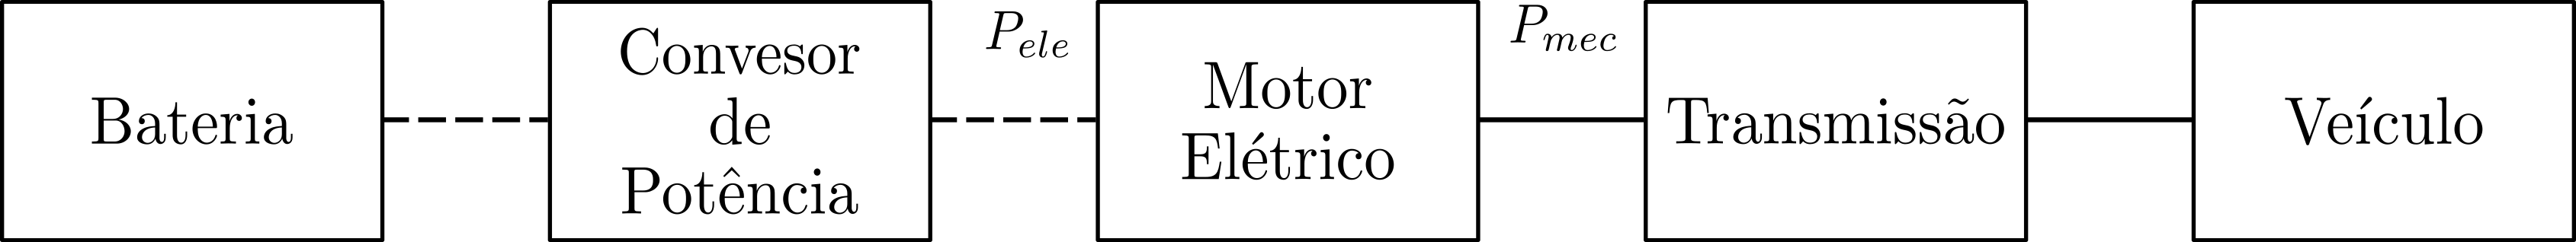
\includegraphics{DescricaoProcesso/Figuras/g874.png}
	\caption*{\footnotesize Fonte: Elaborado pelo autor.}
\end{figure}



Bateria eletroquímica, ou apenas bateria, é um dispositivo em que durante a descarga ocorre a conversão de energia potêncial química em energia
elétrica e na carga ocorre a conversão inversa. Ou seja, uma bateria armazena energia elétrica na forma de energia potêncial química. Uma bateria é
composta por varais células ligadas entre si. Uma célula de bateria é composta por dois elétrodos --- positivo e
negativo --- imersos em um eletrólito. \cite[Seç.~13.1]{book:Modern_Electric_Vehicles}



Conversor eletrônico de potência, ou conversor de potência, é o circuito cujo a finalidade é extrair energia elétrica de um sistema de energia e
transformá-la em uma forma adequada e necessária para um motor. \cite[Cap.~1]{book:Electric_Motor_Control}


O motor elétrico converte a potência elétrica --- tensão e corrente --- em potência mecânica rotativa --- torque e rotação --- para impulsionar o
veículo. \cite[Cap.~7]{book:Modern_Electric_Vehicles} Podem ser classificados em relação a sua alimentação: corrente continua
(CA) ou corrente alternada (CC), conforme apresentado na Figura \ref{classif_motor}.
No entanto o motor de corrente continua sem escovas, ou BLDC do inglês \textit{brushless direct current}, é difícil de ser classificado desse forma
pois sua configuração é semelhante à de um motor CA, enquanto suas características elétricas são semelhantes às de um motor
CC. \cite[Cap.~10]{book:Electric_Motor_Control} Nesse trabalho estudara-se o modelo dos motores BLDC pois é o tipo de motor utilizado no protótipo DT1.

\begin{figure}[h]
	\centering
	\caption{Classificação de motores elétricos}
	\label{classif_motor}
	\begin{tikzpicture}[grow'=right,
			level distance=4cm,
			level 1/.style={sibling distance=5cm},
			level 2/.style={sibling distance=1.5cm},
			edge from parent fork right]
		\tikzstyle{every node}=[draw,minimum width=1in,text width=1in,align=center]

		%\draw [help lines] (0,-5) grid (10,5);

		\node (Root) {Motor Elétrico}
		child {
				node {Corrente Continua}
				child { node {Excitação independente} }
				child { node {Auto excitação} }
			}
		child {
				node {Corrente Alternada}
				child { node {Síncrono} }
				child { node {Assíncrono (indução)} }
			};
		\node[draw] at (8, 0)	(a) {BLDC};
		\draw[dashed] (6,2) -- (6,-2);
		\draw[dashed] (6,0) -- (6.55,0);
	\end{tikzpicture}
	\caption*{\footnotesize Fonte: Adaptado de \citeauthoronline{book:Electric_Motor_Control}. \cite[Cap.~1]{book:Electric_Motor_Control}}
\end{figure}

O motor BLDC foi desenvolvido em 1962 e possui um sistema de comutação eletrônica ao inves de comutação mecânica como os motores CC. Para não utilizar
as escovas da comutação mecânica, os enrolamentos da armadura são colocados no estator (parte estacionaria) e os ímãs são colocados no rotor (parte
rotativa).
A comutação eletrônica baseia-se em sensores para identificar a posição do rotor e acionar o enrolamento necessário para manter o movimento de
rotação. \cite[Cap.~10]{book:Electric_Motor_Control} O conjunto de equações que descreve a corrente de armadura $i_a$ e o torque gerado $T$ para um motor BLDC
de enrolamentos ligados em
Y com neutro acessível e operando em meia onda (a tensão é aplicada entre o terminal de um enrolamento e o neutro) é

\begin{subequations}
	\label{eq:MotorCC}
	\begin{align}
		u - u_{ind}  = L_{a} \cdot \dot i_{a} + R_{a} \cdot i_{a}\enspace, \label{eq:MotorCC_1} \\
		u_{ind} = K_{v} \cdot \omega_{m}\enspace, \label{eq:MotorCC_2}                          \\
		T_m = K_{t} \cdot i_{a} \enspace, \label{eq:MotorCC_3}
	\end{align}
\end{subequations}

em que $u$ é a tensão aplicada, $u_{ind}$ é a tensão induzida, $L_{a}$ e $R_{a}$ são, respectivamente a indutância e a resistência da armadura,
$K_{v}$ é a constante de tensão induzida,
$\omega_{m}$ é a rotação do motor e $K_{t}$ é a constante de torque. A Figura \ref{diag:motoBLDC} apresenta o modelo o circuito de um enrolamento do motor BLDC. \cite[Cap.~6]{book:Permanent_Magnet_Motor}

\begin{figure}[h]
	\centering
	\caption{Circuito equivalente de um motor BLDC}
	\begin{center}
		\begin{circuitikz}
			%\draw [help lines] (-1,-2) grid (9,5);

			% circuito
			\draw (0,3) to[V, i<^=$i_a$, v_=$u$] (0,0);
			\draw (0,3) to[R, l=$R_A$] (3,3);
			\draw (3,3) to[L, l=$L_A$] (4,3);
			\draw (4,3) -- (5,3);
			\draw (5,3) to[V, v_=$u_{ind}$] (5,0);
			\draw (0,0) -- (5,0);

			% motor
			\draw[fill=black] (4.85,0.85) rectangle (5.15,2.15);
			\draw[fill=white] (5,1.5) ellipse (.45 and .45);

			% eixo
			\draw[fill=black] (5.45,1.45) rectangle (6.8,1.55);

			% rotação e torque
			\draw[line width=0.7pt,<-] (5.8,1) arc (-30:30:1);
			\draw[line width=0.7pt,<-] (6.4,1) arc (-30:30:1);

			% anotações
			\draw (5.85,2.2) node {$\omega_m$};
			\draw (6.4,2.25) node {$T$};
			\draw (4.5, 2.25) node {$+$};
			\draw (4.5, 0.75) node {$-$};
		\end{circuitikz}
	\end{center}
	\label{diag:motoBLDC}
	\caption*{\footnotesize Fonte: Elaborado pelo autor.}
\end{figure}

O protótipo DT1 é equipado com um motor Dunkermotoren BG75x75 40V (Figura \ref{fig:motor_bg75}). O motor que possui 3 enrolamentos, imã de neodímio
com 8 polos e sensor hall integrado para medir a posição do rotor (24 pulsos por volta).
% , suas características elétricas e mecânicas estão
% apresentadas na Tabela \ref{tab:dadosBg75}.


	\begin{figure}[H]
		\centering
		\caption{Motor Dunkermotoren BG75x75 40V}
		\label{fig:motor_bg75}
		\includegraphics[scale=0.15]{DescricaoProcesso/Figuras/bg75.png}
		\caption*{\footnotesize Fonte: Equipe Milhagem UFMG}
	\end{figure}

	% \begin{table}[H]
	% 		\centering
	% 		\caption{Dados do motor BG75x75 40V}
	% 		\label{tab:dadosBg75}
	% 		\rowcolors{1}{}{lightgray}
	% 		\begin{tabular}{lcc}
	% 			\toprule
	% 			Tensão nominal            & {[}V{]}        & 40     \\
	% 			Corrente nominal          & {[}A{]}        & 15,6   \\
	% 			Torque nominal            & {[}N.m{]}      & 1,50    \\
	% 			Velocidade nominal        & {[}rpm{]}      & 3370   \\
	% 			Troque de atrito          & {[}N.m{]}      & 0,13   \\
	% 			Torque de parada          & {[}N.m{]}      & 12     \\
	% 			Velocidade sem carga      & {[}rpm{]}      & 4100   \\
	% 			potência de saída nominal & {[}W{]}        & 530    \\
	% 			potência de saída máxima  & {[}W{]}        & 1150   \\
	% 			Constante de torque       & {[}N.m/A{]}    & 0,119  \\
	% 			Resistência               & {[}$\Omega${]} & 0,07   \\
	% 			Indutância                & {[}mH{]}       & 0,45   \\
	% 			Corrente de pico          & {[}A{]}        & 63     \\
	% 			Inercia do rotor          & {[}g.m²{]}     & 0,0625 \\
	% 			Massa                     & {[}kg{]}       & 2,8    \\
	% 			\bottomrule
	% 		\end{tabular}
	% 		\caption*{\footnotesize Fonte: Adaptado de  \citeauthoronline{manual:BG75}. \cite{manual:BG75}}
	% \end{table}

% \begin{multicols*}{2}
% 	\begin{figure}[H]
% 		\centering
% 		\caption{Motor Dunkermotoren BG75x75 40V}
% 		\label{fig:motor_bg75}
% 		\includegraphics[scale=0.15]{DescricaoProcesso/Figuras/bg75.png}
% 		\caption*{\footnotesize Fonte: Equipe Milhagem UFMG}
% 	\end{figure}

% 	%\vfill\null
% 	\columnbreak

% 	\begin{table}[H]
% 		\centering
% 		\caption{Dados do motor BG75x75 40V}
% 		\label{tab:dadosBg75}
% 		\rowcolors{1}{}{lightgray}
% 		\begin{tabular}{lcc}
% 			\toprule
% 			Tensão nominal            & {[}V{]}        & 40     \\
% 			Corrente nominal          & {[}A{]}        & 15,6   \\
% 			Torque nominal            & {[}N.m{]}      & 1,50    \\
% 			Velocidade nominal        & {[}rpm{]}      & 3370   \\
% 			Troque de atrito          & {[}N.m{]}      & 0,13   \\
% 			Torque de parada          & {[}N.m{]}      & 12     \\
% 			Velocidade sem carga      & {[}rpm{]}      & 4100   \\
% 			potência de saída nominal & {[}W{]}        & 530    \\
% 			potência de saída máxima  & {[}W{]}        & 1150   \\
% 			Constante de torque       & {[}N.m/A{]}    & 0,119  \\
% 			Resistência               & {[}$\Omega${]} & 0,07   \\
% 			Indutância                & {[}mH{]}       & 0,45   \\
% 			Corrente de pico          & {[}A{]}        & 63     \\
% 			Inercia do rotor          & {[}g.m²{]}     & 0,0625 \\
% 			Massa                     & {[}kg{]}       & 2,8    \\
% 			\bottomrule
% 		\end{tabular}
% 		\caption*{\footnotesize Fonte: Adaptado de  \citeauthoronline{manual:BG75}. \cite{manual:BG75}}
% 	\end{table}
% \end{multicols*}

A transmissão do veículo regula a transferência de potência do motor para as rodas. É basicamente composta por mecanismo de
redução --- ex. caixa de câmbio --- e por um mecanismo de interrupção --- ex. embreagem. \cite[Cap.~4]{book:Modern_Electric_Vehicles}
No DT1, o mecanismo de redução utilizado é do tipo roda de atrito e o mecanismo de interrupção é o pivotamento entre os componentes da roda de atrito, apresentado na Figura \ref{dig:Trasmissao}.

\begin{figure}[H]
	\centering
	\caption{Representação da transmissão do DT1}
	\label{dig:Trasmissao}
	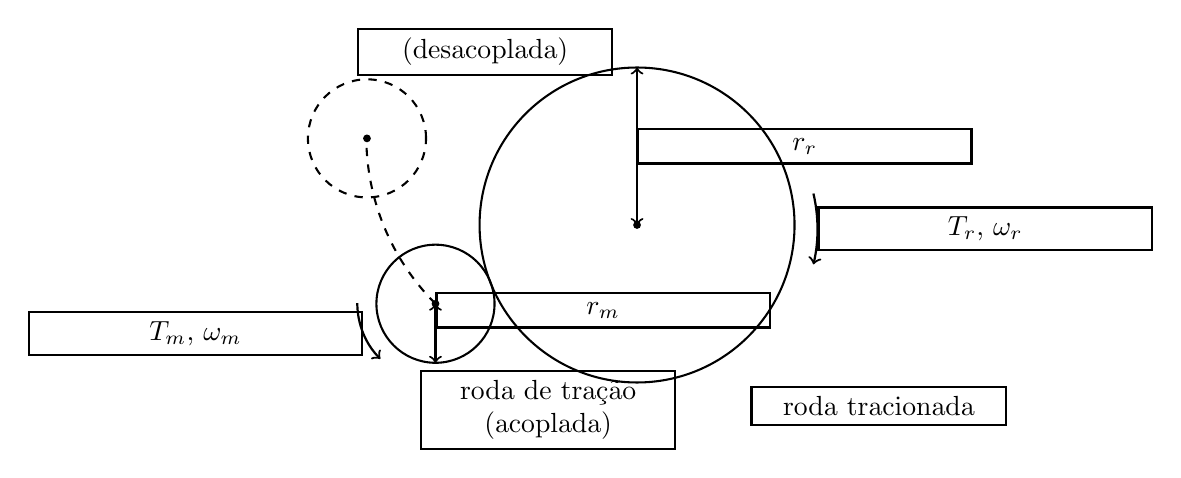
\begin{tikzpicture}
		%\draw [help lines] (-2,-2) grid (6,4);

		\filldraw[black] (0,0) circle (1pt);
		\draw (0,0) circle (0.75cm);
		\draw [thick,<-] (-0.7, -0.7) arc (225:180:1cm) node[pos=0.5, left] {$T_m$, $\omega_m$};
		\draw[<->] (0,0) -- (0,-0.75) node[pos=0.11, right] {$r_{m}$}; 

		\filldraw[black] (-0.87,2.1) circle (1pt);
		\draw [dashed] (-0.87,2.1) circle (0.75cm);

		\filldraw[black] (2.56,1) circle (1pt);
		\draw (2.56,1) circle (2cm);
		\draw[thick,<-] (4.8, 0.5) arc (-13:13:2cm) node[pos=0.5, right] {$T_r$, $\omega_r$};
		\draw[<->] (2.56,1) -- (2.56,3) node[pos=0.5, right] {$r_{r}$}; 

		\draw[dashed] (0, 0) arc (225:180:3cm); 
		\draw (4,-1.3) node[minimum width=3cm,text width=3cm,align=center]{roda tracionada};
		\draw (-0.2,-1.35) node[minimum width=3cm,text width=3cm,align=center]{roda de tração (acoplada)};
		\draw (-1,3.2) node[minimum width=3cm,text width=3cm,align=center]{(desacoplada)};
	\end{tikzpicture}
	\caption*{\footnotesize Fonte: Elaborada pelo autor.}
\end{figure}

Rodas de atrito são uma das maneiras mais simples para se transmitir potência mecânica entre eixos e sua eficiência é tipicamente de $95$ a $98$ {\%}. São compostas por dois ou mais cilindros em contato direto.  
Para não ocorrer deslizamento em uma roda de atrito o torque transmitido não deve exceder a força de atrito entre os cilindros. Os torque e rotações são descritos pelas equações 

\begin{subequations}
	\label{eq:Transmissao}
	\begin{align}
		\varphi = \frac{r_{r}}{r_{m}}\enspace, \label{eq:Transmissao_1} \\
		\omega_{r} = -\frac{\omega_{m}}{\varphi}\enspace, \label{eq:Transmissao_2}  \\
		T_{r} =\varphi \cdot T_{m} \cdot \eta\enspace, \label{eq:Transmissao_3}
	\end{align}
\end{subequations}

onde $\varphi$ é a relação de transmissão, $R_{r}$ e $\omega_{r}$ são o diâmetro e a velocidade angular da roda, 
$R_{m}$ e $\omega_{m}$ são o diâmetro e a velocidade angular do cilindro motor e $\eta$ é a eficiência da roda de atrito. \cite[Seç.~20.4]{book:Niemann1971}\cite[Seç.~9.1]{book:Norton2010}



A partir das Equações (\ref{eq:MotorCC}) e (\ref{eq:Transmissao}), desconsiderando as perdas por atrito visco nos rolamentos, as perdas causada pela resistência interna na bateira e
a perda no conversor de potência, o conjunto que descreve o a força do sistema de propulsão $F_t$ de um veiculo elétrico é

\begin{subequations}
	\label{eq:propulsao}
	\begin{align}
		\dot i_{a} = \frac{u - K_{v} \cdot \omega_{m} - R_{a} \cdot i_{a}}{L_{a}}\enspace, \label{eq:propulsao_1} \\
		F_{t} =  \frac{K_t \cdot i_a \cdot \varphi \cdot \eta}{r_r}\enspace. \label{eq:propulsao_2}
	\end{align}
\end{subequations}

\section{Controle Ótimo}

"O objetivo da teoria de controle ótimo é determinar os sinais de controle que farão com que um processo satisfaça as restrições físicas e ao mesmo
tempo minimize
(ou maximize) alguns critérios de desempenho."~\cite[Cap.~1]{book:Kirk}

\subsection{Introdução teórica}

O conjunto de Equações (\ref{eq:formulacaoOCP}) é uma formulação genérica e comum para um problema de controle ótimo (OCP)


\begin{mini!}
	{x(\cdot),u(\cdot), p, T}{\int_{0}^{T} L(x(t),u(t),p) \,\mathrm{d}t \;+\; E(x(T),p) \label{eq:ObjOCP}}
	{\label{eq:formulacaoOCP}}{}
	\addConstraint{x(0)-x_{0}}{=0 \label{eq:C1_OCP}}{}
	\addConstraint{\dot x(t) - f(x(t),u(t))}{=0, \quad}{t \in \left[0,T\right]  \label{eq:C2_OCP}}
	\addConstraint{h(x(t),u(t))}{\leq 0, \quad}{t \in \left[0,T\right]  \label{eq:C3_OCP}}
	\addConstraint{r(x(T))}{\leq 0 \label{eq:C4_OCP}}{}
	\addConstraint{T }{\leq T_{max} \label{eq:C5_OCP}}{}
	\addConstraint{p_{min}\leq p}{ \leq p_{max} \, \label{eq:C6_OCP}}{}
\end{mini!}

em que a Equação (\ref{eq:ObjOCP}) é o função objetivo, Equação (\ref{eq:C1_OCP}) é uma restrição de estados iniciaisfixos, Equação (\ref{eq:C2_OCP}) é
a restrição
que representa a dinâmica
do sistema, Equação (\ref{eq:C3_OCP}) são restrições de caminho sobre os estados do sistema e sobre as variáveis de controle, Equação (\ref{eq:C4_OCP})
é uma restrição de espaço para os estados finais, Equação (\ref{eq:C5_OCP}) é a restrição para o tempo final e Equação (\ref{eq:C6_OCP}) são restrições de intervalo para parâmetros otimizáveis.
O função objetivo, também conhecido como objetivo de Bolza, é composto por uma integral de $L(x,u)$ conhecida como termo de Lagrange
e uma função $E(x)$ conhecida como termo de Meyer. \cite[Cap.~9]{book:Numerical_Optimal_Control}

A soluçai de um problema de controle ótimo é uma sequência de sinais de controle em malha aberta e um conjunto de paramentos, o comportamento esperado é
exemplificado na Figura \ref{fig:simpleOCP}.

\begin{figure}[H]
	\centering
	\caption{Exemplo do comportamento desejado das variáveis em um OCP}
	\label{fig:simpleOCP}
	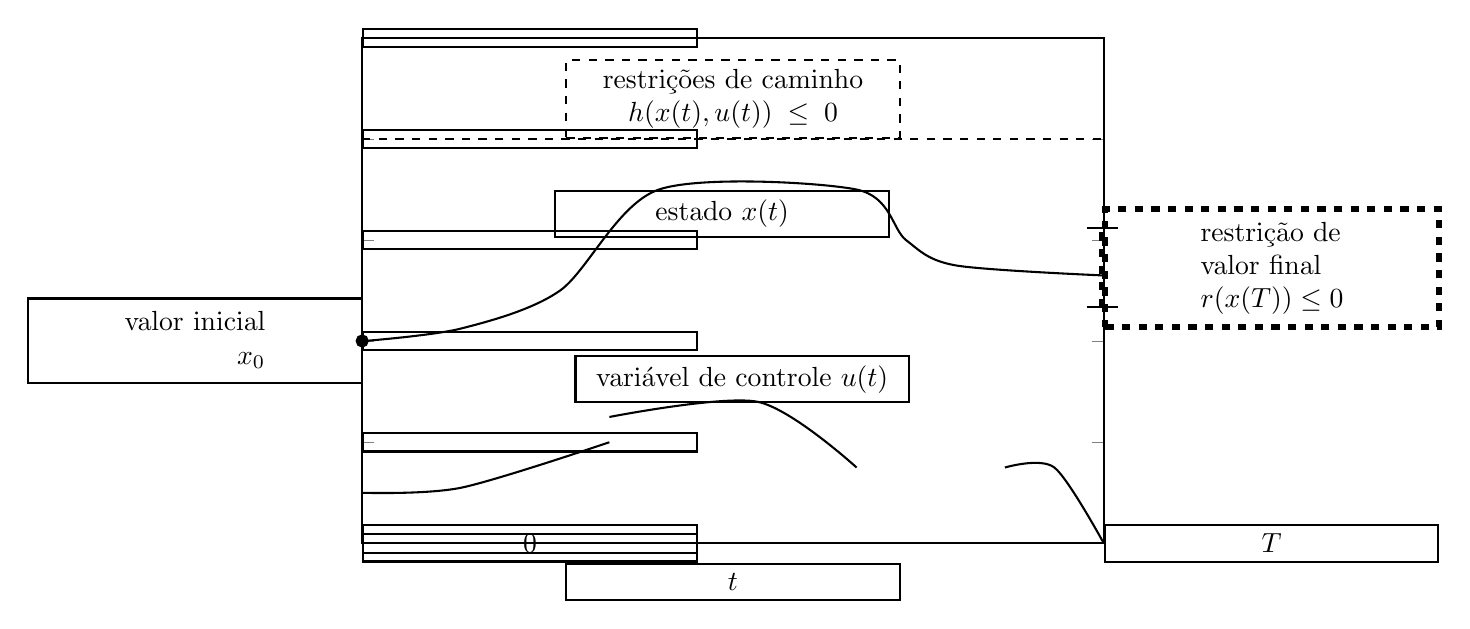
\begin{tikzpicture}
		%\draw [help lines] (-1,-2) grid (12,7);
		\centering
		\begin{axis}[
				width=11cm, height=8cm,
				xmin=0, xmax=15,
				ymin=0, ymax=10,
				xlabel=$t$,
				xtick = {0,15}, xticklabels = {$0$,$T$},
				yticklabels={}]
			\addplot[smooth] plot coordinates {
					(0, 4)
					(2, 4.25)
					(4, 5)
					(6, 7)
					(10, 7)
					(11, 6)
					(12, 5.5)
					(15, 5.3)
				}node[pos=.5, below] {estado $x(t)$};

			\addplot[smooth] plot coordinates {
					(0, 1)
					(2, 1.1)
					(5, 2)
				};
			\addplot[smooth] plot coordinates {
					(5, 2.5)
					(8, 2.8)
					(10, 1.5)
				}node[pos=.5, above] {vari\'{a}vel de controle $u(t)$};
			\addplot[smooth] plot coordinates {
					(10, 0)
					(13, 0)
				};
			\addplot[smooth] plot coordinates {
					(13, 1.5)
					(14, 1.5)
					(15, 0)
				};

			\addplot[dashed, black] coordinates {
					(0,8) (15,8)
				}node[pos=.5, above] {restri\c{c}\~{o}es de caminho $h(x(t),u(t)) \leq 0$};

		\end{axis}
		\filldraw[black] (0,2.57) circle (2pt) node[left] {
				\begin{tabular}{r}
					valor inicial \\$x_0$
				\end{tabular}
			};
		\draw (9.2,3) -- (9.6,3) (9.2,4) -- (9.6,4);
		\draw[dashed,line width=0.75mm] (9.4,3) -- (9.4,4) node[right, pos=.5] {
			\begin{tabular}{l}
				restri\c{c}\~{a}o de \\valor final\\	$r(x(T))\leq 0$
			\end{tabular}
		};
	\end{tikzpicture}
	\caption*{\footnotesize Fonte: Adaptado de \citeauthoronline{book:Numerical_Optimal_Control}. \cite{book:Numerical_Optimal_Control}}
\end{figure}

Segundo \citeauthoronline{article:Diehl}, de forma geral, há três abordagens básicas para solução computacional de um OCP, (a) programação dinâmica, (b) métodos indiretos e (c) métodos diretos, 
conforme apresentado na Figura \ref{fig:diagrama_metodos_numericos}. \cite{article:Diehl}

\begin{enumerate}[(a)]
	\item Programação dinâmica: utiliza o princípio de otimalidade de Bellman (em um caminho ótimo A-B-C os caminhos A-B e B-C também são ótimos) para calcular recursivamente a sequência de controle ótimo. 
	\item Métodos indiretos: utiliza a filosofia "primeiro otimizar e então discretizar", que é escrever as condições de otimalidade contínuas primeiro,
		resultando em um problemas de valor de contorno (sistema de equações diferenciais acrecido de um conjunto adicional de restrições chamadas condições de contorno) e depois discretizá-lo para resolver numericamente.
	\item Métodos diretos: utiliza a filosofia "primeiro discretizar e então otimizar", isto é primeiro discretize as equações do OCP e, em seguida, aplique um algoritmo de otimização para resolver o problema de programação 
	não linear resultante ( NLP do inglês \textit{Nonlinear Programming Problem}) resultante.
\end{enumerate}

Para a solução de OCP em aplicações no mundo real, os métodos diretos são atualmente as técnicas mais difundidas e usadas com sucesso. \cite{article:Diehl,book:betts2010}

Métodos diretos reformulam o OCP da Equação (\ref{eq:formulacaoOCP}) em um problema de programação não linear de dimensão finita (NLP) da forma:

\begin{mini!}
	{w}{a(w) \label{eq: NLP1}}
	{\label{eq: NLP}}{}
	\addConstraint{b(w)}{= 0 \label{eq: NLP2}}{}
	\addConstraint{c(w)}{\geq 0, \label{eq: NLP3}}{}
\end{mini!}

com um vetor de dimensão finita $w$ representando os graus de liberdade de otimização e com funções diferenciáveis $a$ (escalar), $b$ e $c$ (vetores). 
Todos os métodos diretos começam por uma parametrização da variável de controle, mas diferem na forma como os estados são tratados. Podem ser classificados em duas abordagems, sequnciais e simultâneos. \cite{article:Diehl} 

Nas abordagens sequênciais, os estado $x(t)$ são uma função implícita dos controles $u(t)$ e do valor inicial $x_0$. Dessa forma, a simulação
e as iterações de otimização procedem sequêncialmente e o NLP possui apenas o controle discretizado como graus de liberdade de otimização. O método mais usado de abordagem sequêncial é o \textit{Direct Single Shooting}. \cite{article:Diehl}

As abordagens simultâneas fazem uma parametrização dos estado como variáveis de otimização dentro do NLP e adicionam restrições de igualdade que representam a dinâmica do sistema. 
Com isso, a simulação e a otimização ocorrem simultaneamente, e somente na solução do NLP os estados representam uma solução da equação da dinâmica do sistema válida e
correspondente à variável de controle. As duas variações mais comuns da abordagem simultânea são \textit{Direct Multiple Shooting} e \textit{Direct Collocation}. \cite{article:Diehl}

\begin{figure}[h]
	\centering
	\caption{Visão geral dos métodos numéricos para controle ótimo}
	\label{fig:diagrama_metodos_numericos}
	\begin{tikzpicture}[
			level distance=2cm,
			level 1/.style={sibling distance=3.5cm},
			level 2/.style={sibling distance=5.2cm},
			level 3/.style={sibling distance=3.5cm},
			edge from parent fork down
			]
		\tikzstyle{every node}=[draw,minimum width=2.7cm,text width=2.7cm,align=center]

		%\draw [help lines] (0,-5) grid (10,5);

		\node (Root) {Controle Ótimo}
			child {	node {Programação Dinâmica} }
			child {	node {Métodos Indiretos} }
			child { node {Métodos Diretos}
				child { node {Métodos sequênciais} 
					child {	node {\textit{Direct Single Shooting}} }
				}
				child { node {Métodos Simultâneos} 
					child {	node {\textit{Direct Multiple Shooting}} }
					child {	node {\textit{Direct Collocation}} }
				}
			};
	\end{tikzpicture}
	\caption*{\footnotesize Fonte: Adaptado de \citeauthoronline{article:Diehl}. \cite{article:Diehl}}
\end{figure}

\subsection{O \textit{software} FALCON.m}

FALCON.m é um é uma biblioteca de \textit{software}, proprietária de uso gratuito, para MATLAB , 
desenvolvida no \textit{Institute of Flight System Dynamics} da \textit{Technische Universit{\"a}t M{\"u}nchen} para resolução e 
análise de problemas de controle ótimo e estimação de parâmetros utilizando o método \textit{Direct Collocation}. Capaz de resolver grandes problemas de controle ótimo com de até 600 mil variáveis de otimização. \cite{manual:Falcon} \cite[Cap.~4]{phd:Rieck}

Ela segue o paradigma de programação orientada a objetos, um resumo de suas principais classes de objetos é apresentado na Figura \ref{fig:objetosFalcon}. 
A classe \lstinline[style=Matlab-editor]{Problem} é a principal, nela são configurados as fases (\lstinline[style=Matlab-editor]{Phases}) do OCP, os parâmetros otimizáveis, o custo de Mayer e
o método de discretização a ser utilizado . Os métodos de discretização disponíveis na biblioteca são: 
trapezoidal (padrão) ou \textit{backward Euler}.  Na classe \lstinline[style=Matlab-editor]{Phases}, são adicionados o modelo da dinâmica do sistema, os estados, as variáveis 
de controle, as restrições de caminho, o custo de Lagrange e os instantes de tempos inicial e final. \cite[Cap.~4]{phd:Matthias}

A biblioteca utiliza otimizadores para NLP externos, como cada optimizador  tem uma interface única, no momento, é possível  utilizar interfaces para três otmizadores: IPOPT, SNOPT e WORHP. 
O optimizador  utilizado neste trabalho é o IPOPT, configuração pré-definida da biblioteca FALCON.m. Mais informações sobre a utilização do FALCON.m pode ser consultadas em seu manual. \cite{manual:Falcon}
\begin{figure}[h]
	\centering
	\caption{Resumo com principais objetos da biblioteca FALCON.m}
	\label{fig:objetosFalcon}
	\begin{tikzpicture}[%
		grow via three points={one child at (0.5,-0.7) and
		two children at (0.5,-0.7) and (0.5,-1.4)},
		edge from parent path={(\tikzparentnode.south) |- (\tikzchildnode.west)}]
	
		\tikzstyle{every node}=[draw,minimum width=4cm,text width=4cm,align=center, anchor=west]
		\tikzstyle{selected}=[fill=gray!50]
		\tikzstyle{optional}=[dashed,fill=gray!50]
	
		\node [selected] {Problem}
		  child { node [selected] {Phases}
			child { node [selected] {Model}}
			child { node {StateGrid}}
			child { node {ControlGrid}}
			child { node {PathConstraints}}
			child { node {LagrangeCosts}}
			child { node {InitialTime}}
			child { node {FinalTime}}
		  }	
		  child [missing] {}				
		  child [missing] {}				
		  child [missing] {}
		  child [missing] {}				
		  child [missing] {}				
		  child [missing] {}	
		  child [missing] {}	
		  child { node {Parameters}}
		  child { node {MayerCosts}}
		  child { node {DiscretizationMethod}};
	\end{tikzpicture}
	\caption*{\footnotesize Fonte: Adaptado de \citeauthoronline{phd:Matthias}. \cite{phd:Matthias}}
\end{figure}

\subsubsection{IPOPT}

O projeto COIN-OR, do inglês \textit{COmputational INfrastructure for Operations Research},
 é uma iniciativa que visa promover \textit{software} de código aberto para a comunidade de pesquisa operacional. \cite{article:CoinOr} 
 Dentre as bibliotecas disponibilizadas no projeto COIN-OR está a IPOPT, do inglês \textit{Interior Point OPTimizer}.
 Escrita em C++ e Fortran para solução de problemas de otimização não linear (NLP) utilizando o
 método de pontos interiores com filtro apresentado por \citeauthoronline{article:Ipopt}. Sua licença é a EPL que permite uso gratuito e acesso ao código. Mais detalhes sobre está biblioteca podem ser obtidos na pagina do seu repositório no GitHub  \url{https://github.com/coin-or/Ipopt}.

\clearpage